\chapter{Kurzfassung}

\par

\includegraphics[scale = 0.46]{purity}

\par
\textbf{Problem}: Sei $(A, D(A))$ Generator einer $C_0$-Halbgruppe auf einem Banachraum $X$ und $(B, D(B))$ ein weiterer Operator auf $X$. Unter welchen Bedingungen ist $A+B$, oder eine Fortsetzung $K$ von $A+B$, Generator einer $C_0$ Halbgruppe auf $X$?

\par
% 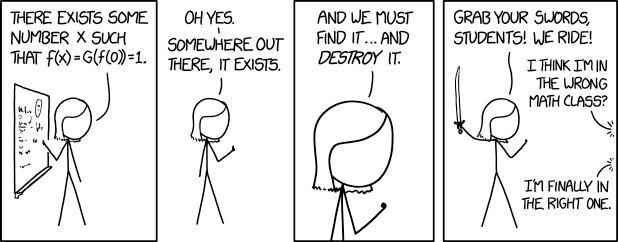
\includegraphics[scale = 0.55]{existence_proof}

% An dieser Stelle steht eine Zusammenfassung der Arbeit, Umfang
% max.\ 1 Seite. Im Unterschied zu anderen Kapiteln ist die
% Kurzfassung (und das Abstract) üblicherweise nicht in Abschnitte
% und Unterabschnitte gegliedert. 
% Auch Fußnoten sind hier falsch am Platz.

% Kurzfassungen werden übrigens häufig -- zusammen mit Autor und Titel
% der Arbeit -- %
% in Literaturdatenbanken aufgenommen. Es ist daher darauf zu
% achten, dass die Information in der Kurzfassung für sich 
% \emph{allein} (\dah ohne weitere Teile der Arbeit) zusammenhängend und
% abgeschlossen ist. Insbesondere werden an dieser Stelle (wie \ua
% auch im \emph{Titel} der Arbeit und im \emph{Abstract})
% normalerweise \emph{keine Literaturverweise} verwendet! Falls man
% unbedingt solche benötigt -- etwa weil die Arbeit eine
% Weiterentwicklung einer bestimmten, früheren Arbeit darstellt --,
% dann sind \emph{vollständige} Quellenangaben in der Kurzfassung
% selbst notwendig, \zB %
% [\textsc{Zobel} J.: \textit{Writing for Computer Science -- The Art of
% Effective Commu\-nica\-tion}. Springer-Verlag, Singa\-pur, 1997].

% Weiters sollte man daran denken, dass bei der Aufnahme in Datenbanken
% Sonderzeichen oder etwa Aufzählungen mit "`Knödellisten"' in der
% Regel verloren gehen. Dasselbe gilt natürlich auch für das 
% \emph{Abstract}.


% Inhaltlich sollte die Kurzfassung \emph{keine} Auflistung der
% einzelnen Kapitel sein (dafür ist das Einleitungskapitel
% vorgesehen), sondern dem Leser einen kompakten, inhaltlichen
% Überblick über die gesamte Arbeit verschaffen. Der hier verwendete
% Aufbau ist daher zwangsläufig anders als der in der Einleitung.
